\documentclass[11pt]{article}

% --- Packages ---
\usepackage[margin=1in]{geometry}
\usepackage{amsmath, amssymb, amsthm, mathtools}
\usepackage{booktabs}
\usepackage{hyperref}
\usepackage{enumitem}
\usepackage{tikz}
\usetikzlibrary{arrows.meta, positioning, calc}

% --- Theorem environments ---
\newtheorem{theorem}{Theorem}
\newtheorem{lemma}{Lemma}
\newtheorem{proposition}{Proposition}
\theoremstyle{definition}
\newtheorem{definition}{Definition}
\newtheorem{remark}{Remark}

% --- Macros ---
\newcommand{\Poly}{\mathbf{Poly}}
\newcommand{\Set}{\mathbf{Set}}
\newcommand{\WAgent}{\mathsf{WAgent}}
\newcommand{\Either}{\mathsf{Either}}
\newcommand{\Maybe}{\mathsf{Maybe}}
\newcommand{\Err}{\mathsf{Err}}
\newcommand{\Tok}{\mathsf{Token}}
\newcommand{\Approval}{\mathsf{Approval}}
\newcommand{\San}{\mathsf{Sanitize}}
\newcommand{\Val}{\mathsf{Validate}}
\newcommand{\Exec}{\mathsf{Exec}}
\newcommand{\Obs}{\mathsf{Obs}}
\newcommand{\Act}{\mathsf{Act}}

\title{\textbf{Biological Motifs for Agentic Control}\\
\large A Functorial Bridge between Gene Regulatory Networks and Autonomous Software Architectures}
\author{Bogdan Banu\\\texttt{bogdan@banu.be}}
\date{December 9, 2025}

\begin{document}
\maketitle

% ==========================================
% ABSTRACT
% ==========================================
\begin{abstract}
The transition of Large Language Models (LLMs) from passive generators to autonomous agents has introduced significant challenges in reliability, security, and state management. Current agentic architectures are often constructed ad-hoc, prone to ``hallucination cascades,'' infinite loops, and prompt injection attacks. This paper proposes that these failure modes are not unique to software but are instances of universal control problems solved by biological systems over billions of years. We present a formal isomorphism between Gene Regulatory Networks (GRNs) and Agentic Software Systems using \textbf{Applied Category Theory}. We model agents as \textbf{Polynomial Functors} within the category $\Poly$, and their interactions via the \textbf{Operad of Wiring Diagrams}. We derive a rigorous syntax for agent composition by mapping biological mechanisms---including \textit{Quorum Sensing} for consensus, \textit{Chaperone Proteins} for structural validation, and \textit{Endosymbiosis} for neuro-symbolic integration---to software design patterns. This framework provides a mathematical basis for ``Epigenetic'' state management (RAG) and the topological defense against adversarial ``Prion'' attacks.
\end{abstract}

\section{Introduction}

Artificial Intelligence is shifting from \emph{Generative AI} (single-shot text generation) to \emph{Agentic AI}
(systems that execute multi-step workflows to achieve goals). While individual LLM capabilities scale
predictably, engineering \emph{systems of agents} remains fragile. Developers face non-deterministic
outputs, runaway loops, adversarial instructions, and the challenge of maintaining global coherence
under partial observability and stochastic behavior.

We argue these challenges are not unique to software. They are fundamental constraints of distributed
information processing. A close analogue to a multi-agent architecture is a \emph{Gene Regulatory Network}
(GRN): thousands of genes read local signals and express proteins that regulate other genes, producing
robust behavior under noise, resource constraints, and adversarial environments.

\subsection{The Biological Heuristic}

Systems biology identifies recurring \emph{network motifs} that implement control functions (filtering,
memory, consensus, and defense). We focus on four motifs that map naturally to agentic engineering:

\begin{itemize}[leftmargin=*]
  \item \textbf{Coherent Feed-Forward Loop (CFFL):} persistence detection and gating, analogous to
  two-key execution guardrails.
  \item \textbf{Quorum sensing:} distributed consensus via thresholded aggregation, analogous to
  ensemble voting with confidence thresholds.
  \item \textbf{Chaperone-assisted folding:} structural validation and repair loops, analogous to schema
  validation and retry mechanisms.
  \item \textbf{Immune-like self-defense:} mechanisms distinguishing trusted signals from untrusted
  inputs, analogous to prompt-injection containment and information-flow policies.
\end{itemize}

\subsection{From Metaphor to Discipline}

To make the analogy actionable, we use Applied Category Theory:
polynomial functors in $\Poly$ represent \emph{typed open interfaces}, and wiring diagrams represent
\emph{compositional structure}. We emphasize an important precision:

\begin{quote}
We do \emph{not} claim GRNs and agentic systems are identical in physics or implementation.
We claim they admit a shared \emph{interface-level semantics} in $\Poly$ that supports compositional
reasoning about wiring, validation, gating, and resource control.
\end{quote}

\subsection{Contributions}

\begin{enumerate}[leftmargin=*]
  \item \textbf{A Formal Dictionary:} a rigorous correspondence between biological components
  (genes, promoters, plasmids) and software components (agents, schemas, tools).
  \item \textbf{A Safer Agentic Operad $\WAgent$:} a syntax for agent wiring with types, integrity labels,
  and effect tracking, supporting compile-time rejection of ill-formed compositions.
  \item \textbf{Correct Topological Safety Claims:} topology enforces \emph{interlocks}, not independence;
  we provide the correct probabilistic statement for CFFL safety and the corresponding design
  requirements for independence/diversity.
  \item \textbf{A Pathology Lens:} agentic failures are analyzed as dysregulated network dynamics,
  informing termination, validation, and security treatments.
\end{enumerate}


\section{Related Work}

This work sits at the intersection of Systems Biology, Applied Category Theory, and Agentic AI.

\subsection{Network Motifs in Systems Biology}

Network motifs as statistically over-represented subgraphs were introduced by Milo et al.
Their functional characterization, including feed-forward persistence detection, is developed further
by Alon.

\subsection{Applied Category Theory (ACT)}

We use the categorical language of open dynamical systems, polynomial functors, and wiring-diagram
operads (e.g., Spivak; Vagner--Spivak--Lerman) to formalize interface composition.

\subsection{Reliability in Agentic AI}

Techniques such as iterative self-critique and reasoning loops improve output quality but typically act
at the prompt level rather than at the topology level. We propose that reliability can be designed as a
property of architecture: gating, validation, resource budgets, and information-flow constraints.


\section{The Bridge: GRNs and Agents as Open Interfaces in \texorpdfstring{$\Poly$}{Poly}}

To relate GRNs and agentic systems, we map both to a common mathematical representation:
polynomial functors for interfaces and coalgebras for stateful behavior.

\subsection{Preliminaries: Polynomial Functors}

\begin{definition}[Polynomial Functor]
A (finitary) polynomial functor $P$ is an object of $\Poly$ of the form
\begin{equation}
  P(y) \;=\; \sum_{o \in O} y^{I(o)} .
  \label{eq:poly}
\end{equation}
Here $O$ is a set of \emph{positions} (outputs). For each $o \in O$, $I(o)$ is the set of
\emph{directions} (inputs) enabled/required after emitting $o$.
\end{definition}

Intuitively, a system exposes an output $o$ and then awaits an input $i \in I(o)$ before proceeding.

\begin{figure}[h]
\centering
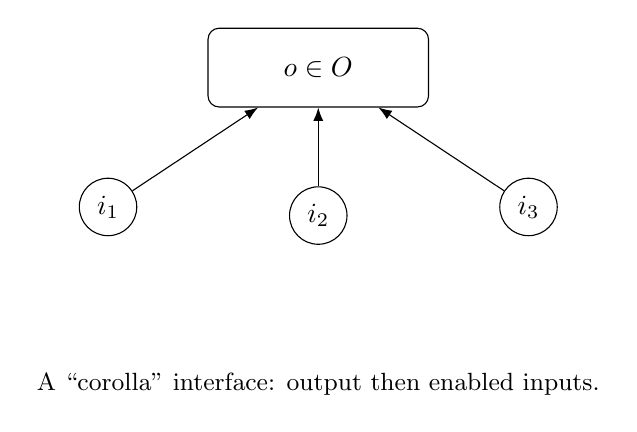
\begin{tikzpicture}[>=Latex, node distance=10mm]
  \node[draw, rounded corners, minimum width=28mm, minimum height=10mm] (cap) {$o \in O$};
  \node[draw, circle, below left=10mm and 10mm of cap] (i1) {$i_1$};
  \node[draw, circle, below=10mm of cap] (i2) {$i_2$};
  \node[draw, circle, below right=10mm and 10mm of cap] (i3) {$i_3$};
  \draw[->] (i1) -- (cap);
  \draw[->] (i2) -- (cap);
  \draw[->] (i3) -- (cap);
  \node[below=15mm of i2] {\small A ``corolla'' interface: output then enabled inputs.};
\end{tikzpicture}
\caption{A visual mnemonic for a polynomial interface.}
\end{figure}

\subsection{Coalgebras: Stateful Open Systems}

\begin{definition}[Coalgebra for $P$]
A (deterministic) open dynamical system with interface $P$ is a coalgebra $(S,\varphi)$ where
\begin{equation}
  \varphi: S \to P(S).
  \label{eq:coalgebra}
\end{equation}
Expanding $P(S)=\sum_{o\in O} S^{I(o)}$, the structure map yields:
(1) a \emph{readout} selecting an output position $o$, and
(2) an \emph{update} selecting next state given an input direction.
\end{definition}

This is the level at which both GRNs and agentic systems admit a shared description: state $S$,
interface $P$, and compositional wiring.

\subsection{Two Domain Categories and Two Encodings}

We make the scope of the correspondence explicit.

\begin{definition}[Interface Categories (Sketch)]
Let $\mathbf{GRN}_{\mathrm{int}}$ be a category whose objects are \emph{open regulatory modules}
with typed signal ports, and whose morphisms are admissible couplings (regulatory connections)
that respect those ports. Let $\mathbf{AG}_{\mathrm{int}}$ be a category whose objects are \emph{open agent
modules} with typed I/O ports, and whose morphisms are admissible dataflow connections.
\end{definition}

\begin{proposition}[Encodings into $\Poly$ (Informal)]
There exist interface encodings (functors)
\[
  F: \mathbf{GRN}_{\mathrm{int}} \to \Poly
  \qquad\text{and}\qquad
  G: \mathbf{AG}_{\mathrm{int}} \to \Poly
\]
that map each module to a polynomial interface and each admissible coupling to a morphism in $\Poly$.
\end{proposition}

\begin{remark}
We do not claim $\mathbf{GRN}_{\mathrm{int}} \cong \mathbf{AG}_{\mathrm{int}}$ as categories.
Instead, we claim both admit a faithful \emph{interface-level} representation in $\Poly$ under the
chosen abstraction (typed ports, open composition, and stateful coalgebra semantics).
\end{remark}

\subsection{Genes and Agents as Polynomial Interfaces}

The original presentation used uniform direction sets, which is too coarse for both domains.
We refine the definitions by allowing \emph{position-dependent directions}.

\begin{definition}[Gene Interface Object]
Fix a gene/module $G$. Let $O_G$ be the set of possible expression outcomes (e.g., protein isoforms,
expression regimes, or ``off''), and for each $o\in O_G$ let $I_G(o)$ be the set of regulatory contexts
(binding configurations, signal tuples) that are meaningful after $o$ is selected.
Define:
\begin{equation}
  P_G(y) \;=\; \sum_{o \in O_G} y^{I_G(o)} .
  \label{eq:gene-poly}
\end{equation}
\end{definition}

\begin{definition}[Agent Interface Object]
Fix an agent module $A$. Let $O_A$ be the set of action-positions (e.g., respond to user, call tool
$\kappa$, request clarification, emit approval token, terminate), and for each $o\in O_A$ let $I_A(o)$
be the expected observation type(s) after taking action $o$.
Define:
\begin{equation}
  P_A(y) \;=\; \sum_{o \in O_A} y^{I_A(o)} .
  \label{eq:agent-poly}
\end{equation}
\end{definition}

This refinement matches reality: different actions induce different expected next observations; and
different gene expression regimes correspond to different relevant regulatory inputs.

\subsection{Promoters and Schemas as \emph{Validated} Optics (Not ``Undefined'')}

In biology, a promoter gates what signals are relevant to a gene. In software, schemas and context
windows gate what data is visible and how it is interpreted. The crucial correction is that mismatches
should not be treated as ``mathematically undefined''; they should be modeled as \emph{partial} or
\emph{effectful} maps with explicit error values.

\begin{definition}[Validated Lens (Sketch)]
A validated lens from global state $S$ to local view $V$ is a pair
\[
  \mathrm{get}: S \to \Either(\Err, V),
  \qquad
  \mathrm{put}: S \times V' \to S,
\]
where $\mathrm{get}$ may fail with an error value when the promoter/schema does not match.
\end{definition}

\begin{remark}
This aligns with real agent systems: a schema mismatch typically triggers error handling, retries,
or safe termination, rather than an ``undefined'' computation.
\end{remark}

\subsection{Epigenetics and Memory as State}

Both domains are stateful:
epigenetic markers bias gene responsiveness without changing DNA, while RAG/history bias agent
behavior without changing model weights. In our coalgebra semantics, these correspond to the internal
state $S$.

\subsection{Dictionary}

\begin{table}[h]
\centering
\small
\begin{tabular}{@{}lll@{}}
\toprule
Category Concept & Biological Realization (GRN) & Software Realization (Agentic)\\
\midrule
Polynomial functor $P$ & Module interface & Agent/module interface\\
Position set $O$ & Expression outcomes & Action kinds (tool call, reply, stop, \dots)\\
Directions $I(o)$ & Regulatory contexts & Expected next observation types\\
Validated lens & Promoter gating & Schema/context gating with error handling\\
State $S$ & Epigenetic landscape & Memory/RAG/history\\
Morphisms & Signal transduction wiring & Dataflow wiring\\
\bottomrule
\end{tabular}
\caption{A compositional dictionary at the interface level.}
\end{table}


\section{A Formal Syntax for Agent Composition: The Operad \texorpdfstring{$\WAgent$}{WAgent}}

We now define a wiring discipline for agentic systems that supports:
(1) static rejection of ill-typed wiring,
(2) explicit validation boundaries, and
(3) information-flow and capability reasoning.

\subsection{Data Types, Integrity Labels, and Capabilities}

\begin{definition}[Base Data Types]
Let $\mathcal{T}$ be a set of base data types, e.g.
\[
  \mathcal{T} = \{\mathsf{Text},\, \mathsf{JSON}(\Sigma),\, \mathsf{Image},\, \mathsf{ToolCall}(\kappa),\, \mathsf{Error},\, \mathsf{Stop},\, \Approval\}.
\]
\end{definition}

\begin{definition}[Integrity Labels]
Let $\mathcal{L}=\{\mathsf{U},\mathsf{V},\mathsf{T}\}$ denote integrity levels:
\[
  \mathsf{U}=\text{untrusted},\quad
  \mathsf{V}=\text{validated},\quad
  \mathsf{T}=\text{trusted}.
\]
We order them $\mathsf{U} \le \mathsf{V} \le \mathsf{T}$ and enforce \emph{integrity-preserving flow}:
a wire may connect output label $\ell_{\mathrm{out}}$ to input label $\ell_{\mathrm{in}}$ only if
\begin{equation}
  \ell_{\mathrm{out}} \ge \ell_{\mathrm{in}}.
  \label{eq:integrity-flow}
\end{equation}
Thus untrusted data cannot directly feed a trusted-required port.
\end{definition}

\begin{definition}[Capabilities / Effects]
Let $\mathcal{C}$ be a set of capabilities (effects), e.g.
\[
  \mathcal{C}=\{\mathsf{ReadFS},\mathsf{WriteFS},\mathsf{Net},\mathsf{ExecCode},\mathsf{Money},\mathsf{EmailSend}\}.
\]
Each box (agent/module) carries an effect set $\epsilon \subseteq \mathcal{C}$, and composition
aggregates effects by union unless restricted by a policy.
\end{definition}

\subsection{Ports and Well-Formed Wiring}

\begin{definition}[Port Type]
A port carries a \emph{decorated type} $(\tau,\ell)$ where $\tau\in\mathcal{T}$ and $\ell\in\mathcal{L}$.
(Effects are box-level annotations, but may be required by specific ports such as execution.)
\end{definition}

\begin{definition}[Well-Typed Wire]
A wire from port $(\tau_1,\ell_1)$ to port $(\tau_2,\ell_2)$ is well-typed when:
\[
  \tau_1 = \tau_2
  \quad\text{and}\quad
  \ell_1 \ge \ell_2.
\]
\end{definition}

\begin{remark}
This is the core distinction between \emph{structural correctness} and semantic correctness.
$\WAgent$ can prevent structural integration errors (wrong types, wrong trust boundaries) but cannot,
by itself, guarantee the semantic truth of a text produced by an LLM.
\end{remark}

\subsection{Primitive Composition Operations}

The operad provides three key wiring primitives.

\subsubsection{Parallel Composition $(\otimes)$}

Two agents $A$ and $B$ execute in parallel. Parallel composition is safe when they do not race on a
shared mutable resource, or when shared resources are mediated by explicit resource boxes (locks,
transactions, CRDTs, etc.).

\subsubsection{Serial Composition $(\circ)$}

The output of $A$ feeds the input of $B$. In $\WAgent$, ill-typed connections are rejected at design time.
This moves \emph{structural mismatch failures} (e.g., feeding text into a JSON port) from runtime to
architecture time. It does \emph{not} eliminate semantic hallucinations.

\subsubsection{Feedback / Trace $\mathrm{Tr}$}

Feedback loops represent agency and self-reference, but require termination governance.
Rather than appealing to an undefined ``contractive map'' property, we introduce an explicit progress
measure and budget.

\begin{definition}[Guarded Trace (Fuel/Budget)]
A guarded trace $\mathrm{Tr}_B(A)$ wires feedback through a budget box $B$ that enforces:
(1) a maximum number of iterations and/or tokens, and
(2) a decreasing ranking/progress measure unless external evidence increases it.
\end{definition}


\section{Motif 1: Coherent Feed-Forward Loop and Correct Safety Claims}

\subsection{CFFL as Two-Key Execution}

A coherent feed-forward loop has a direct path and an indirect approval path. In agentic systems,
we treat the indirect path as a verifier producing an explicit approval token.

\begin{figure}[h]
\centering
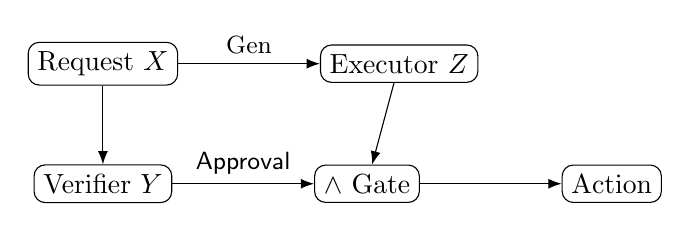
\begin{tikzpicture}[>=Latex, node distance=12mm]
  \node[draw, rounded corners] (X) {Request $X$};
  \node[draw, rounded corners, right=18mm of X] (Z) {Executor $Z$};
  \node[draw, rounded corners, below=10mm of X] (Y) {Verifier $Y$};
  \node[draw, rounded corners, right=18mm of Y] (AND) {$\wedge$ Gate};
  \node[draw, rounded corners, right=18mm of AND] (OUT) {Action};

  \draw[->] (X) -- node[above]{\small Gen} (Z);
  \draw[->] (X) -- (Y);
  \draw[->] (Y) -- node[above]{\small $\Approval$} (AND);
  \draw[->] (Z) -- (AND);
  \draw[->] (AND) -- (OUT);
\end{tikzpicture}
\caption{CFFL as two-key execution: executor output is gated by an approval token.}
\end{figure}

\subsection{The Correct Failure Probability}

We now correct a common but subtle mistake: \emph{an AND gate does not enforce independence}.
It enforces conjunction (both signals required). Independence is an assumption about how errors arise.

\begin{definition}[Error Events]
Let $E_{\mathrm{gen}}$ be the event that the generator/executor path proposes an unsafe or incorrect
action. Let $E_{\mathrm{ver}}$ be the event that the verifier \emph{approves} that unsafe/incorrect action
(i.e., fails to block it).
\end{definition}

\begin{theorem}[CFFL Risk Expression]
In a direct serial execution (no gating), the system fails whenever $E_{\mathrm{gen}}$ occurs:
\[
  \mathbb{P}(\mathrm{Fail}_{\mathrm{direct}}) = \mathbb{P}(E_{\mathrm{gen}}).
\]
In a CFFL with an approval gate, the system fails only when both occur:
\begin{equation}
  \mathbb{P}(\mathrm{Fail}_{\mathrm{CFFL}})
  = \mathbb{P}(E_{\mathrm{gen}} \cap E_{\mathrm{ver}})
  = \mathbb{P}(E_{\mathrm{gen}})\,\mathbb{P}(E_{\mathrm{ver}} \mid E_{\mathrm{gen}}).
  \label{eq:cffl-risk}
\end{equation}
If the verifier catches generator errors with probability $q$, i.e.
$\mathbb{P}(E_{\mathrm{ver}} \mid E_{\mathrm{gen}})=1-q$, then CFFL reduces failure probability
by a factor $(1-q)$ relative to the direct link.
\end{theorem}

\begin{proof}
Direct execution has no second check, so failure is exactly $E_{\mathrm{gen}}$.
In the CFFL, the executor can act only if an approval token is present, so failure requires
(1) an unsafe proposal and (2) verifier approval. The probability identity
$\mathbb{P}(A\cap B)=\mathbb{P}(A)\mathbb{P}(B\mid A)$ yields \eqref{eq:cffl-risk}.
\end{proof}

\begin{remark}[What Topology Guarantees vs What It Does Not]
Topology guarantees an \emph{interlock}: unilateral generator output cannot execute without verifier
approval. Topology does \emph{not} guarantee $\mathbb{P}(E_{\mathrm{ver}} \mid E_{\mathrm{gen}})$ is small.
Reducing that conditional probability requires design choices: model diversity, independent evidence,
tool-based verification, and adversarial testing.
\end{remark}

\subsection{A Topological Guarantee: Two-Key Execution in \texorpdfstring{$\WAgent$}{WAgent}}

\begin{lemma}[Two-Key Execution]
Assume the action sink requires an input port of type $(\Approval,\mathsf{T})$.
Assume the generator path cannot output $(\Approval,\mathsf{T})$ (it outputs at most
$(\mathsf{Text},\mathsf{U})$ or $(\mathsf{ToolCall}(\kappa),\mathsf{V})$).
Then any well-typed wiring diagram that reaches the action sink must include a verifier box that
produces $(\Approval,\mathsf{T})$.
\end{lemma}

\begin{proof}
By $\WAgent$ typing, the action sink must be fed by a wire with exactly the required type and label.
Since the generator cannot produce that port, the only way to satisfy the typing constraints is to
include a box whose output includes $(\Approval,\mathsf{T})$, i.e.\ the verifier.
\end{proof}

\section{Motif 2: Quorum Sensing (Consensus \& Voting)}

Quorum sensing aggregates many weak signals into a robust threshold decision. In agents, this maps to
ensembles and voting.

\begin{remark}[Correlation Warning]
Voting improves reliability when individual errors are not perfectly correlated and when at least a
plurality is better than chance. Shared prompts, shared context poisoning, or a shared misconception
can make errors highly correlated, producing ``confidently wrong'' consensus.
\end{remark}

\paragraph{Design Implication.}
To make quorum useful, inject diversity (different models/temperatures/prompts), incorporate
tool-grounded checks, and consider robust aggregators (weighted voting, abstention, proof-carrying
verifiers).

\section{Motif 3: Chaperones as Partial Validators (Not Retractions)}

Biological chaperones do not implement a perfect inverse; they attempt folding, detect failures,
and route for repair or degradation. The correct software analogue is \emph{partial validation} with
explicit error values.

\begin{definition}[Chaperone Validator (Kleisli Form)]
A chaperone is a Kleisli morphism
\[
  \Val: (\mathsf{Text},\mathsf{U}) \to \Either(\Err, (\mathsf{JSON}(\Sigma),\mathsf{V})).
\]
It either yields a validated structured value or an error trace used for repair.
\end{definition}

\paragraph{Retry \& Repair Loop.}
The generator proposes a structure; the chaperone validates; if invalid, the error is fed back with
bounded retries and a budget box.

\section{Failure Modes as Pathology}

Catastrophic failures often arise not from a single broken component but from dysregulated dynamics.

\subsection{Oncology: Infinite Loops as Unchecked Growth}

\paragraph{Agentic Pathology.}
Agents can enter recursive politeness loops or self-debug loops.

\paragraph{Correct Categorical Diagnosis.}
The problem is not ``distance goes to zero'' in an unspecified metric space. The problem is absence of a
well-founded progress measure and enforced budgets.

\paragraph{Treatment.}
Introduce a guarded trace with:
(1) a step/token budget, and
(2) a ranking function $m(S)\in \mathbb{N}$ that must decrease unless new external evidence arrives.
If $m$ fails to decrease for $k$ steps, trigger apoptosis (termination) or escalation.

\subsection{Autoimmunity: Hallucination Cascades as Integrity Failure}

\paragraph{Agentic Pathology.}
One agent hallucinates; another consumes it from shared memory as if trusted.

\paragraph{Diagnosis.}
This is an integrity-labeling failure: the system does not distinguish untrusted generated text from
validated tool outputs.

\paragraph{Treatment.}
Use integrity labels in $\WAgent$:
tool outputs may be labeled $\mathsf{T}$ (trusted), while generated hypotheses remain $\mathsf{U}$ unless
validated. Require critical decisions to consume $\mathsf{V}$ or $\mathsf{T}$ inputs only.

\subsection{Prion Disease: Prompt Injection as Instruction Contamination}

\paragraph{Agentic Pathology.}
A malicious instruction enters context and influences downstream behavior.

\paragraph{Correct Mechanism Statement.}
Propagation is primarily due to \emph{context mixing and instruction-following} across trust boundaries,
not ``pure geometry'' alone.

\paragraph{Diagnosis.}
An information-flow policy is violated: untrusted text affects privileged control decisions.

\paragraph{Treatment.}
\begin{itemize}[leftmargin=*]
  \item \textbf{Noninterference by construction:} require privileged actions to be gated by
  $(\Approval,\mathsf{T})$ tokens and/or tool-grounded evidence.
  \item \textbf{Sanitization layers:} $\San: (\mathsf{Text},\mathsf{U}) \to (\mathsf{Text},\mathsf{U})$ that removes
  tool-like syntax, policy-violating directives, or embedded prompts (useful but not sufficient alone).
  \item \textbf{Capability least-privilege:} restrict which boxes possess capabilities like $\mathsf{Net}$,
  $\mathsf{WriteFS}$, or $\mathsf{Money}$; require explicit escalation paths.
\end{itemize}

\subsection{Ischemia: Resource Exhaustion}

\paragraph{Agentic Pathology.}
Token starvation, rate limits, latency spikes.

\paragraph{Diagnosis.}
Every wiring-diagram operation consumes resources. Static reasoning can bound \emph{structural} fan-out
and maximum loop iterations, but dynamic effects (model variability, tool delays) require runtime
enforcement.

\paragraph{Treatment.}
A resource-aware runtime enforces token budgets and timeouts. The compiler can reject architectures
that contain \emph{unguarded} trace, but cannot in general compute exact bounds for unconstrained
LLM-driven stopping conditions.


\section{Discussion: Towards ``Epigenetic'' Software}

\subsection{RAG as Digital Methylation}

Treat model weights as static ``DNA'' and RAG/context as epigenetic markers that expose or silence
capabilities.

\[
  O_{\mathrm{agent}} = f(W, E, Q),
\]
where $E$ is an epigenetic state (retrieved documents, memory, policies) shaping behavior without
changing $W$.

\subsection{Horizontal Gene Transfer: Dynamic Tool Loading}

Tool schemas can be injected at runtime like plasmids:
\[
  A_{\mathrm{new}} = A_{\mathrm{old}} \otimes \mathrm{ToolSchema}.
\]
In $\WAgent$, the new schema adds new typed ports and capabilities, and must be mediated by integrity
and effect policies.

\subsection{Metabolic Bounds: What Can Be Guaranteed}

\begin{itemize}[leftmargin=*]
  \item \textbf{Compiler guarantees:} reject unguarded feedback, enforce type/label constraints,
  enforce explicit budget boxes on loops, bound fan-out structurally.
  \item \textbf{Runtime guarantees:} enforce token/time/tool-call budgets, enforce capability limits,
  and trigger safe termination/escalation.
\end{itemize}

\subsection{Endosymbiosis: Neuro-Symbolic Integration}

LLMs excel at planning/semantics but are inefficient at exact arithmetic and formal reasoning.
Integrating deterministic runtimes (REPLs, solvers) yields a symbiotic system:
\[
  A_{\mathrm{euk}} = A_{\mathrm{LLM}} \oplus A_{\mathrm{runtime}}.
\]
In $\WAgent$, the runtime box has sharply typed ports and produces high-integrity outputs
(e.g.\ $(\mathsf{JSON}(\Sigma),\mathsf{T})$), which can then drive high-stakes decisions.


% ==========================================
% 7. CONCLUSION
% ==========================================
\section{Conclusion}

The transition from ``Prompt Engineering'' to ``Agentic Engineering'' represents a shift from alchemy to chemistry. However, current methodologies remain fragile, relying on trial-and-error prompting rather than rigorous architectural principles.

In this paper, we have demonstrated that \textbf{Gene Regulatory Networks (GRNs)} provide a proven architectural blueprint for distributed, stochastic information processing. By formalizing this analogy through \textbf{Applied Category Theory}, we have derived a suite of robust design patterns:

\begin{enumerate}
    \item \textbf{Robustness:} The use of \textit{Quorum Sensing} and \textit{CFFL} topologies to filter stochastic noise.
    \item \textbf{Validity:} The use of \textit{Chaperone Proteins} to enforce structural determinism on probabilistic outputs.
    \item \textbf{Security:} The identification of \textit{Prion-like} prompt injections and the topological defenses required to stop them.
    \item \textbf{Evolution:} The mapping of \textit{Horizontal Gene Transfer} to dynamic tool loading and \textit{Endosymbiosis} to neuro-symbolic integration.
\end{enumerate}

We conclude that the future of reliable AI agents lies in \textbf{biomimetic topology}. By structuring our software according to the logic of life---from the metabolic constraints of Ischemia to the symbiotic integration of code and intuition---we inherit the billions of years of R\&D that biology has invested in solving the problem of autonomous control.


\newpage
\nocite{*}
\bibliographystyle{plain}
\bibliography{references}

\end{document}
